\documentclass[runningheads]{llncs}

\usepackage[T1]{fontenc}
\usepackage{graphicx}
\usepackage{booktabs}
\usepackage{array}
\usepackage{amsmath}
\usepackage{amssymb}
\usepackage{url}
\usepackage{multirow}
\usepackage{enumitem}
\graphicspath{{figures/}}

\begin{document}

\title{Implementable Compressed-Block Storage for Full-State Quantum Circuit Simulation}
\titlerunning{Compressed-Block Storage for Quantum Simulation}

\author{Daniel Adri{\'a}n Gonz{\'a}lez Buend{\'i}a \and
Pablo Josue Rojas Yepes \and
Gilberto Javier D{\'i}az Toro}
\authorrunning{D. Gonz{\'a}lez Buend{\'i}a et al.}

\institute{Universidad Industrial de Santander, Bucaramanga, Colombia}

\maketitle

\begin{abstract}
Full-state quantum circuit simulation remains the reference method for exact execution because every amplitude of the $n$-qubit register is represented explicitly. Its limiting resource is memory: the state vector contains $2^n$ complex amplitudes, so the storage requirement grows exponentially with the number of qubits. Compression is attractive in this setting, but it is useful for live simulation only when the compressed representation is the primary storage format during execution rather than an external persistence mechanism.

This paper presents an implementable compressed-memory architecture for full-state simulators. The design keeps the simulator interface at the level of a logical dense state vector while storing the physical state as independent compressed blocks, a bounded cache of dense materializations, and metadata that controls block authority, writeback, and recovery. The paper specifies the state partition, block descriptor, cache state machine, synchronization rules, and block-acquisition protocol required to execute gates over compressed storage. It also derives the block-access conditions induced by gate stride and shows how single-qubit and controlled operations can be routed through intra-block and inter-block execution plans.

The result is a storage architecture that a simulator developer can implement directly: it identifies which structures must exist, which transitions are legal, when recompression occurs, and how logical state semantics are preserved while dense residency remains bounded.

\keywords{Quantum circuit simulation \and Full-state simulation \and Compressed memory \and State vector \and Memory management}
\end{abstract}

\section{Introduction}

Exact state-vector simulation is still the most direct way to validate quantum circuits, verify compiler transformations, inspect intermediate amplitudes, and compare software and hardware executions. In this model, an $n$-qubit register is represented as
\begin{equation}
  |\psi\rangle = \sum_{i=0}^{2^n-1} \alpha_i |i\rangle,
\end{equation}
with one complex amplitude for each computational basis state~\cite{Nielsen2010}. A double-precision implementation therefore needs
\begin{equation}
  M_{\mathrm{dense}} = 16 \cdot 2^n \text{ bytes}
\end{equation}
just for the state array. This storage cost dominates practical full-state simulation even in optimized simulators such as QuEST and ProjectQ~\cite{Jones2019,Steiger2018,Haner2017,diaz_mdpi_mmss}.

Compression-based simulation addresses the same bottleneck from a different angle: instead of replacing the state-vector model, it attempts to store amplitude data more compactly~\cite{wu2019full,wu2018amplitude,Zhang2025BMQSim}. That direction is useful only if compressed storage participates in the execution path. If gate kernels still require a permanently dense global array, then compression reduces checkpoint or output size, but not the dense working set that constrains simulation.

The central systems problem is therefore not merely how to compress amplitudes, but how to execute state-vector simulation while the primary physical representation is compressed. An implementation needs clear answers to the following questions.
\begin{itemize}[leftmargin=1.4em]
  \item How is the logical state mapped to compressed storage units?
  \item When a gate needs amplitudes, which blocks are materialized and for how long?
  \item What metadata determines whether the compressed payload or the cached dense copy is authoritative?
  \item When can a block be evicted, and when must it be recompressed first?
  \item How does the backend expose a dense programming model to the simulator while managing a compressed physical layout internally?
\end{itemize}

This paper answers those questions with a block-based storage architecture meant to be implemented directly. The contribution is the storage contract itself: the backend structures, invariants, block transitions, and gate-access protocol that make compressed execution practical while preserving the semantics of a dense state vector.

The design is guided by four principles.
\begin{enumerate}[leftmargin=1.5em]
  \item The simulator continues to address a logical dense vector.
  \item The backend owns compression, decompression, cache management, and writeback.
  \item Dense memory is reserved for the current working set rather than for the whole register.
  \item Every legal backend transition preserves one authoritative version of each logical block.
\end{enumerate}

The rest of the paper develops the architecture from the storage model upward: first the logical-to-physical mapping, then the block metadata and cache state machine, then the gate planning rules needed to drive execution through those structures.

\section{Execution Model and Backend Contract}

A compressed backend must preserve the exact same logical state semantics as a conventional dense backend. The simulator therefore interacts with a \emph{logical state vector}, while the backend maintains a \emph{physical state} optimized for bounded residency.

\subsection{Logical State}

The logical state is indexed exactly as in a dense simulator. Basis-state numbering, endianness conventions, gate semantics, amplitude reads, and state export all operate over the same logical ordering used by a conventional state vector. From the simulator's perspective, an access to amplitudes $\alpha_i$ and $\alpha_j$ is still an access to those logical positions, regardless of how the backend stores them internally.

\subsection{Physical State}

The physical state is the implementation-owned representation. It contains:
\begin{itemize}[leftmargin=1.4em]
  \item a partition of the logical vector into contiguous blocks of amplitudes,
  \item one compressed payload per block,
  \item a bounded cache for dense materializations of recently used blocks, and
  \item metadata for block mapping, cache placement, authority, and writeback.
\end{itemize}

Figure~\ref{fig:architecture} summarizes this separation. The simulator emits operations over logical amplitudes; the backend translates those operations into block acquisition, dense execution, dirty marking, eviction, and recompression.

\begin{figure}
  \centering
  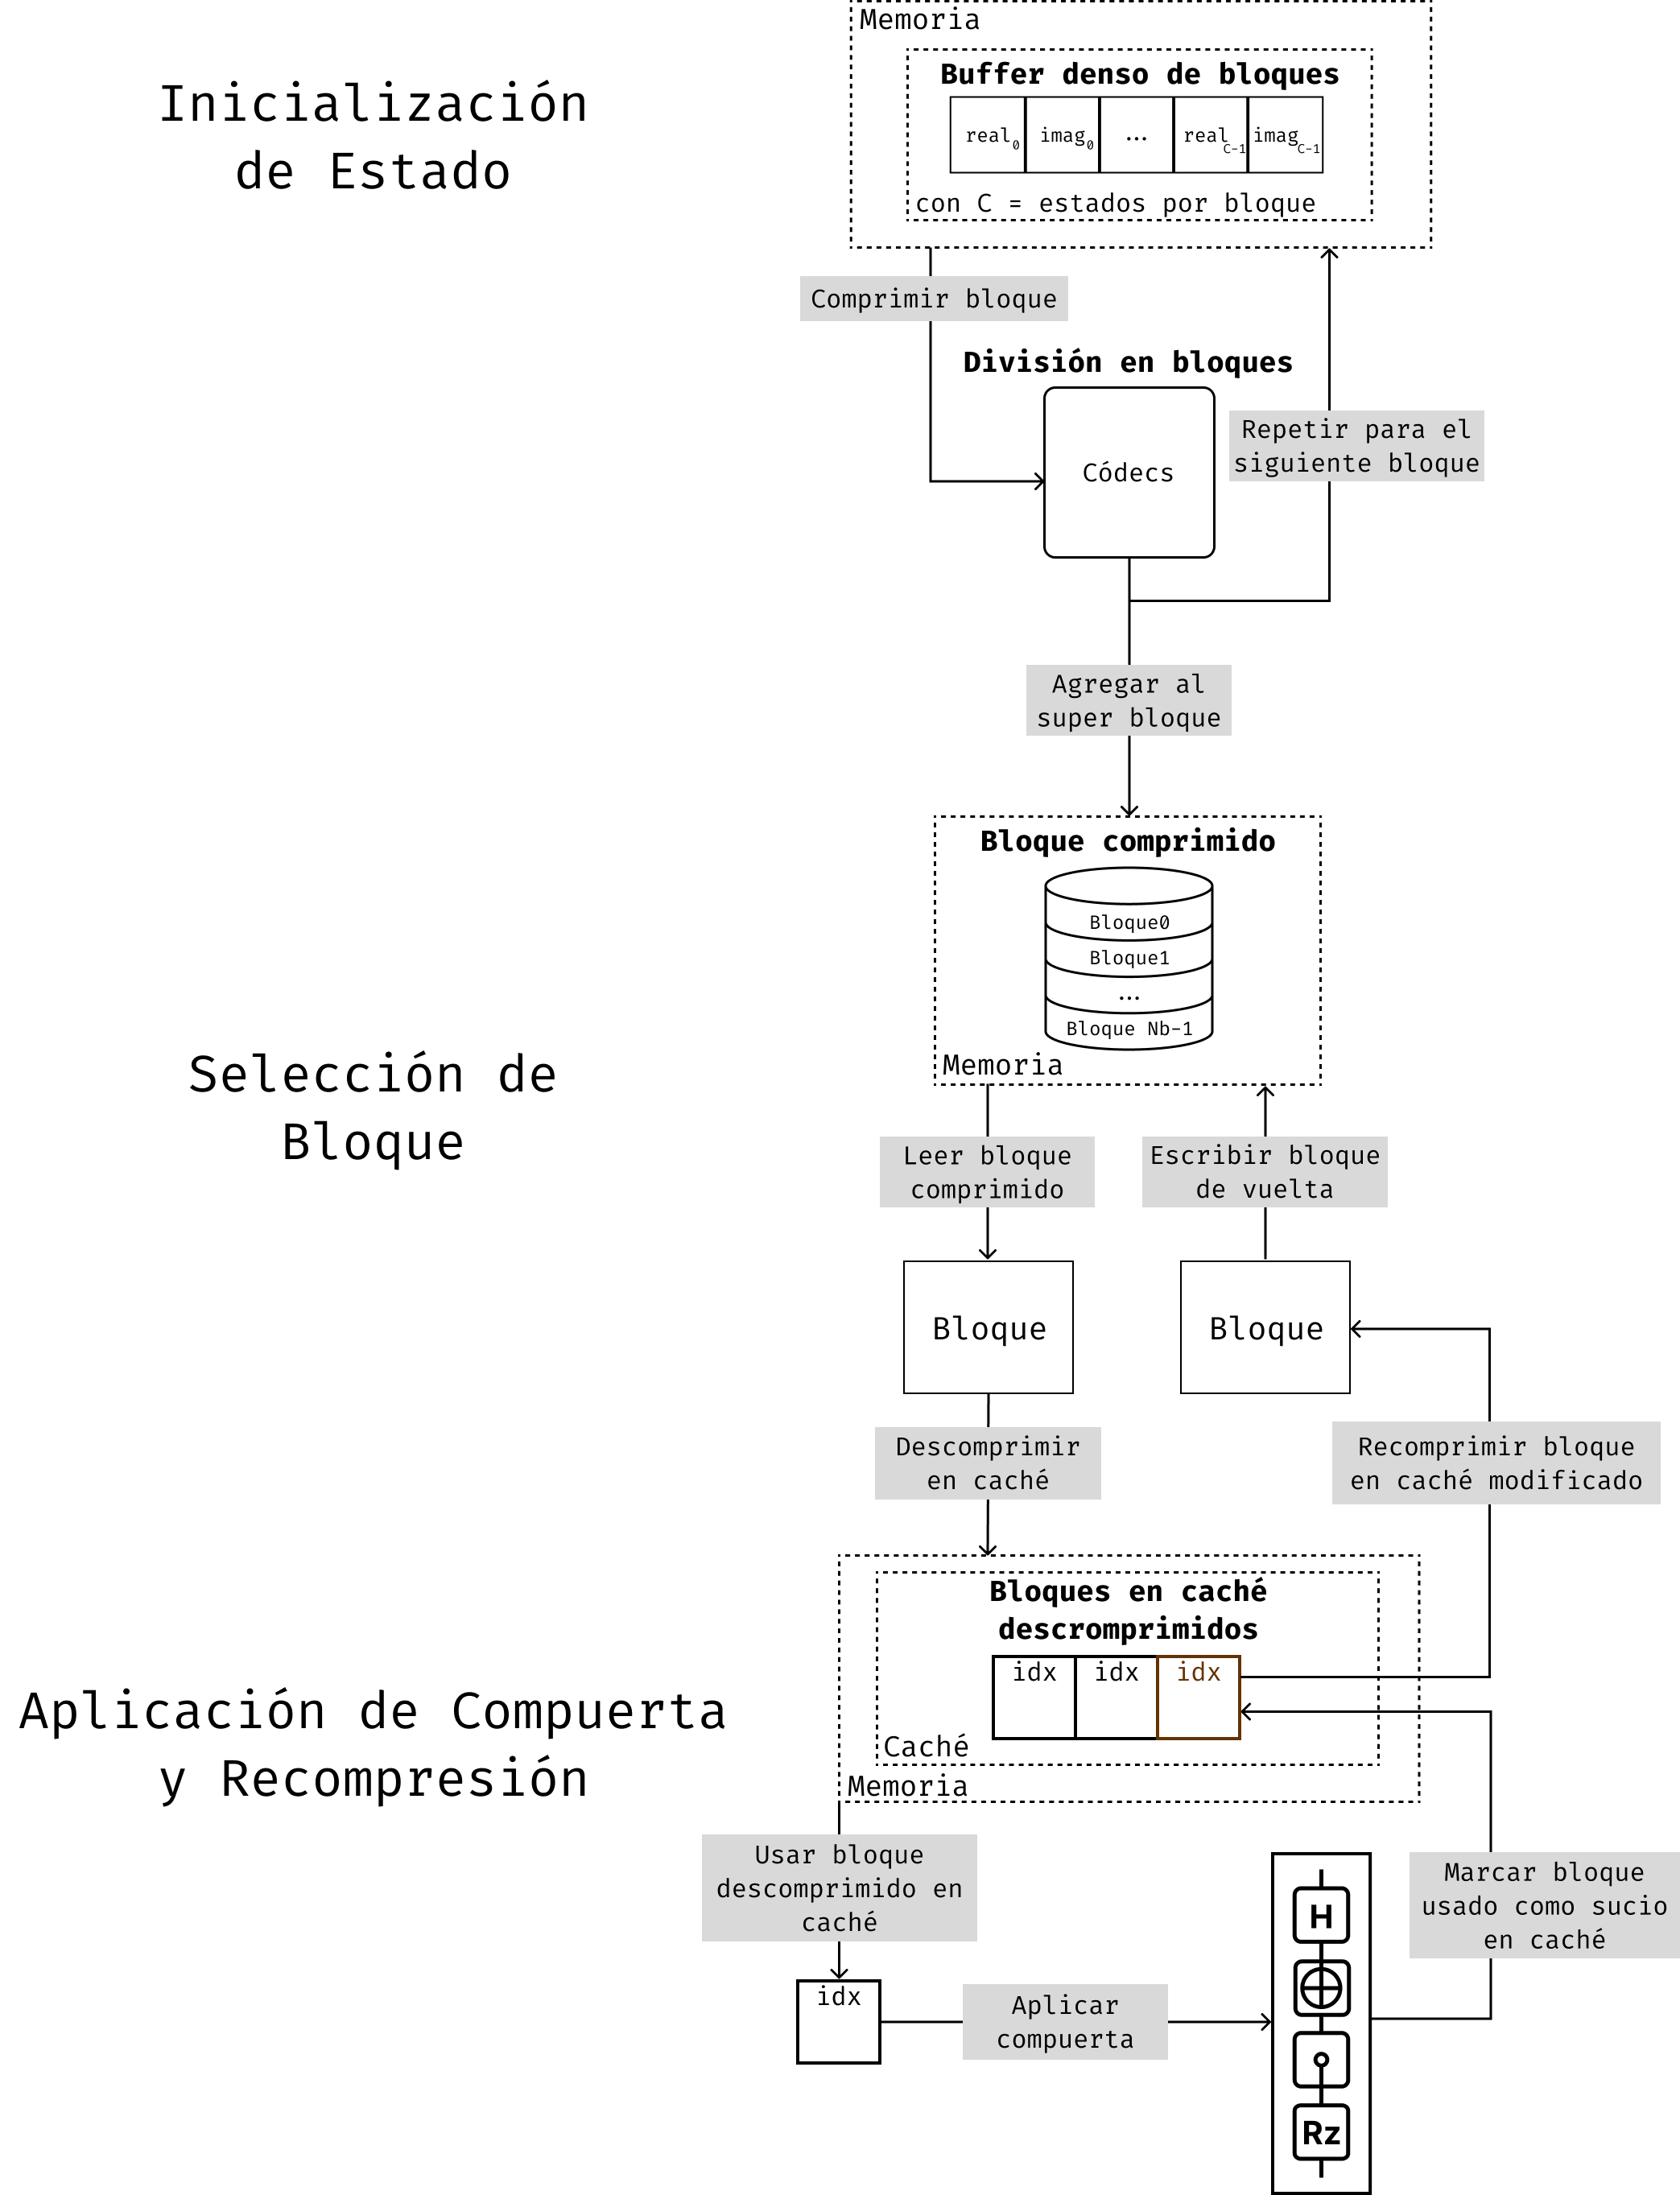
\includegraphics[width=\textwidth]{architecture.png}
  \caption{Compressed-block backend for a full-state simulator. Logical state access remains unchanged at the simulator level; the backend resolves each access through block mapping, dense materialization, and compressed persistence.}
  \label{fig:architecture}
\end{figure}

\subsection{Required Backend Operations}

An implementation only needs a compact set of operations, but those operations must be precise.

\begin{table}
\centering
\caption{Backend operations required to execute over compressed blocks.}
\label{tab:backend-ops}
\begin{tabular}{p{.24\textwidth}p{.66\textwidth}}
\toprule
\textbf{Operation} & \textbf{Responsibility} \\
\midrule
Initialize state & Create block payloads for basis, zero, or externally supplied states. \\
Plan access & Determine which logical blocks a gate instance needs. \\
Acquire block(s) & Ensure that required blocks are resident in dense form and return mutable dense views. \\
Apply kernel & Execute the dense numerical kernel over the acquired block views. \\
Mark dirty & Record that a materialized block now contains newer data than its compressed payload. \\
Flush block(s) & Recompress dirty materializations and update the compressed store. \\
Export state & Flush pending dirty blocks and emit amplitudes in canonical logical order. \\
\bottomrule
\end{tabular}
\end{table}

These operations define the backend contract. Everything else is an implementation detail built on top of them.

\section{State Partition and Block Metadata}

\subsection{Partitioning the Logical Vector}

Let $B$ be the number of amplitudes per block. The logical vector is divided into contiguous regions of size $B$, with the last region shorter if $2^n$ is not a multiple of $B$. Logical amplitude $\alpha_i$ maps to block
\begin{equation}
  j(i)=\left\lfloor \frac{i}{B} \right\rfloor
\end{equation}
and local offset
\begin{equation}
  o(i)= i \bmod B.
\end{equation}
The pair $(j(i), o(i))$ is the only mapping needed to route a logical index into the storage layer. Figure~\ref{fig:block-layout} shows the layout.

\begin{figure}
  \centering
  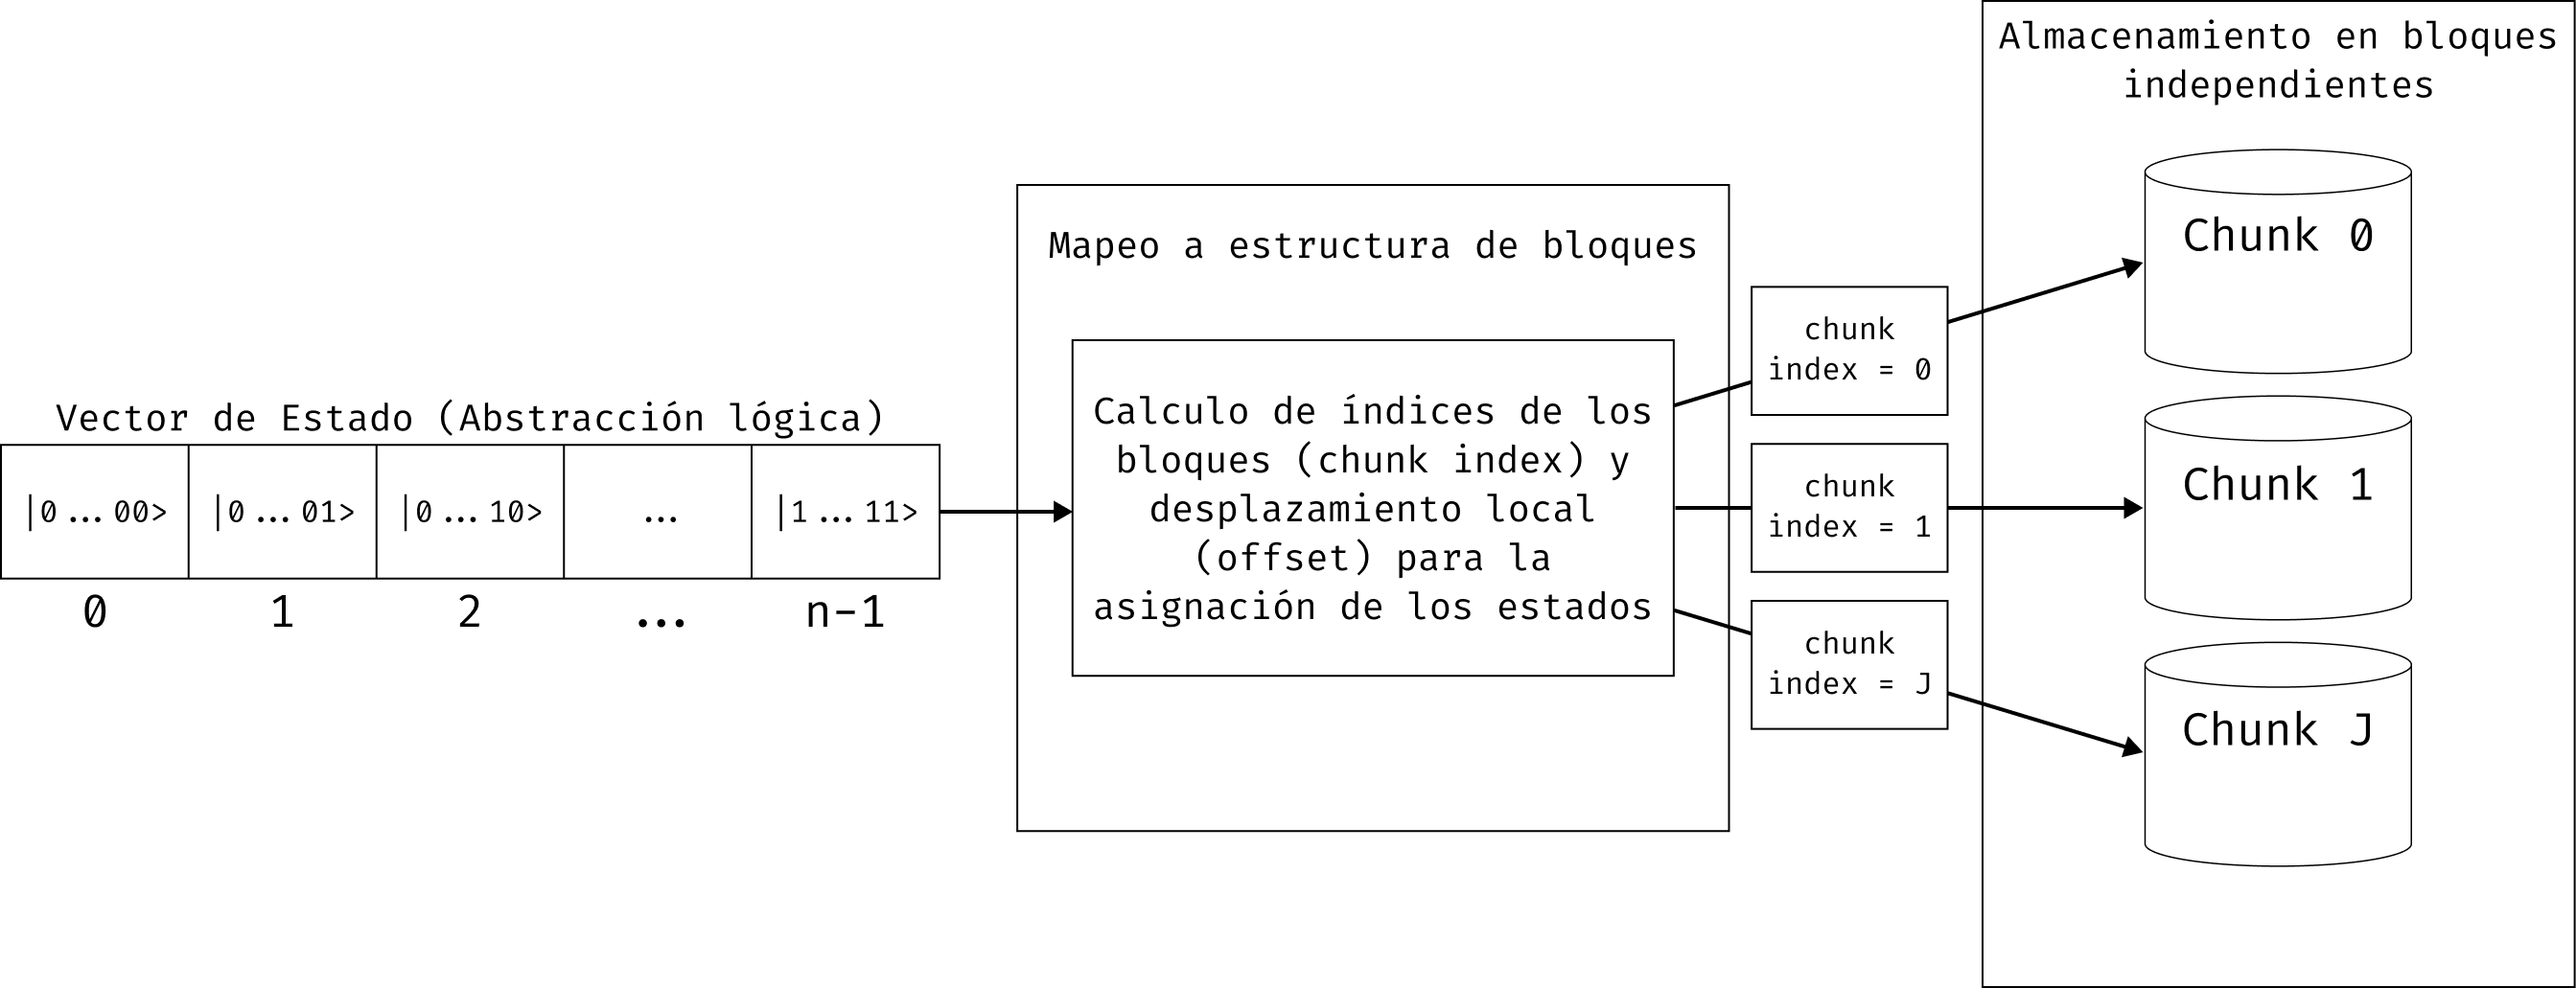
\includegraphics[width=.93\textwidth]{block-layout.png}
  \caption{Contiguous partition of the logical state vector into independently stored blocks. Each logical amplitude index is routed to one block identifier and one local offset.}
  \label{fig:block-layout}
\end{figure}

The block size is part of the execution model, not just a storage parameter. It controls three effects simultaneously: the granularity of compression, the amount of data recovered on a cache miss, and the probability that a gate can execute entirely within one materialized block.

\subsection{Block Descriptor}

Each block is represented by a descriptor held in backend metadata. A practical implementation can store the descriptor as a struct or record with the fields in Table~\ref{tab:block-descriptor}.

\begin{table}
\centering
\caption{Minimal metadata stored for each logical block.}
\label{tab:block-descriptor}
\begin{tabular}{p{.24\textwidth}p{.16\textwidth}p{.48\textwidth}}
\toprule
\textbf{Field} & \textbf{Type} & \textbf{Purpose} \\
\midrule
block\_id & integer & Logical block identifier $j$. \\
logical\_size & integer & Number of valid amplitudes in the block. \\
offset\_bytes & integer & Location of the compressed payload in the backing store. \\
payload\_bytes & integer & Compressed payload length. \\
cache\_slot & integer / null & Dense cache slot if materialized. \\
state & enum & One of \texttt{COMPRESSED}, \texttt{CACHED\_CLEAN}, \texttt{CACHED\_DIRTY}. \\
last\_use & integer / timestamp & Replacement-policy information. \\
codec\_tag & integer / enum & Codec or preprocessing configuration used for this payload. \\
\bottomrule
\end{tabular}
\end{table}

The descriptor belongs to the backend, not to the simulator. Gate kernels should never observe or modify these fields directly.

\subsection{Authoritative Representation}

The compressed backend relies on one strict ownership rule.

\textbf{Authority rule.} Every logical block has exactly one authoritative representation at any time:
\begin{itemize}[leftmargin=1.4em]
  \item when the block state is \texttt{COMPRESSED} or \texttt{CACHED\_CLEAN}, the compressed payload is authoritative;
  \item when the block state is \texttt{CACHED\_DIRTY}, the dense cache slot is authoritative.
\end{itemize}

This rule eliminates ambiguity during recovery and writeback. The backend never needs to reconcile two competing versions of the same logical block.

\section{Cache State Machine and Legal Transitions}

The dense cache stores only currently useful block materializations. The cache may be implemented as a fixed-size array of block buffers plus policy metadata, for example an LRU queue. Figure~\ref{fig:lru-cache} illustrates the intended behavior.

\begin{figure}
  \centering
  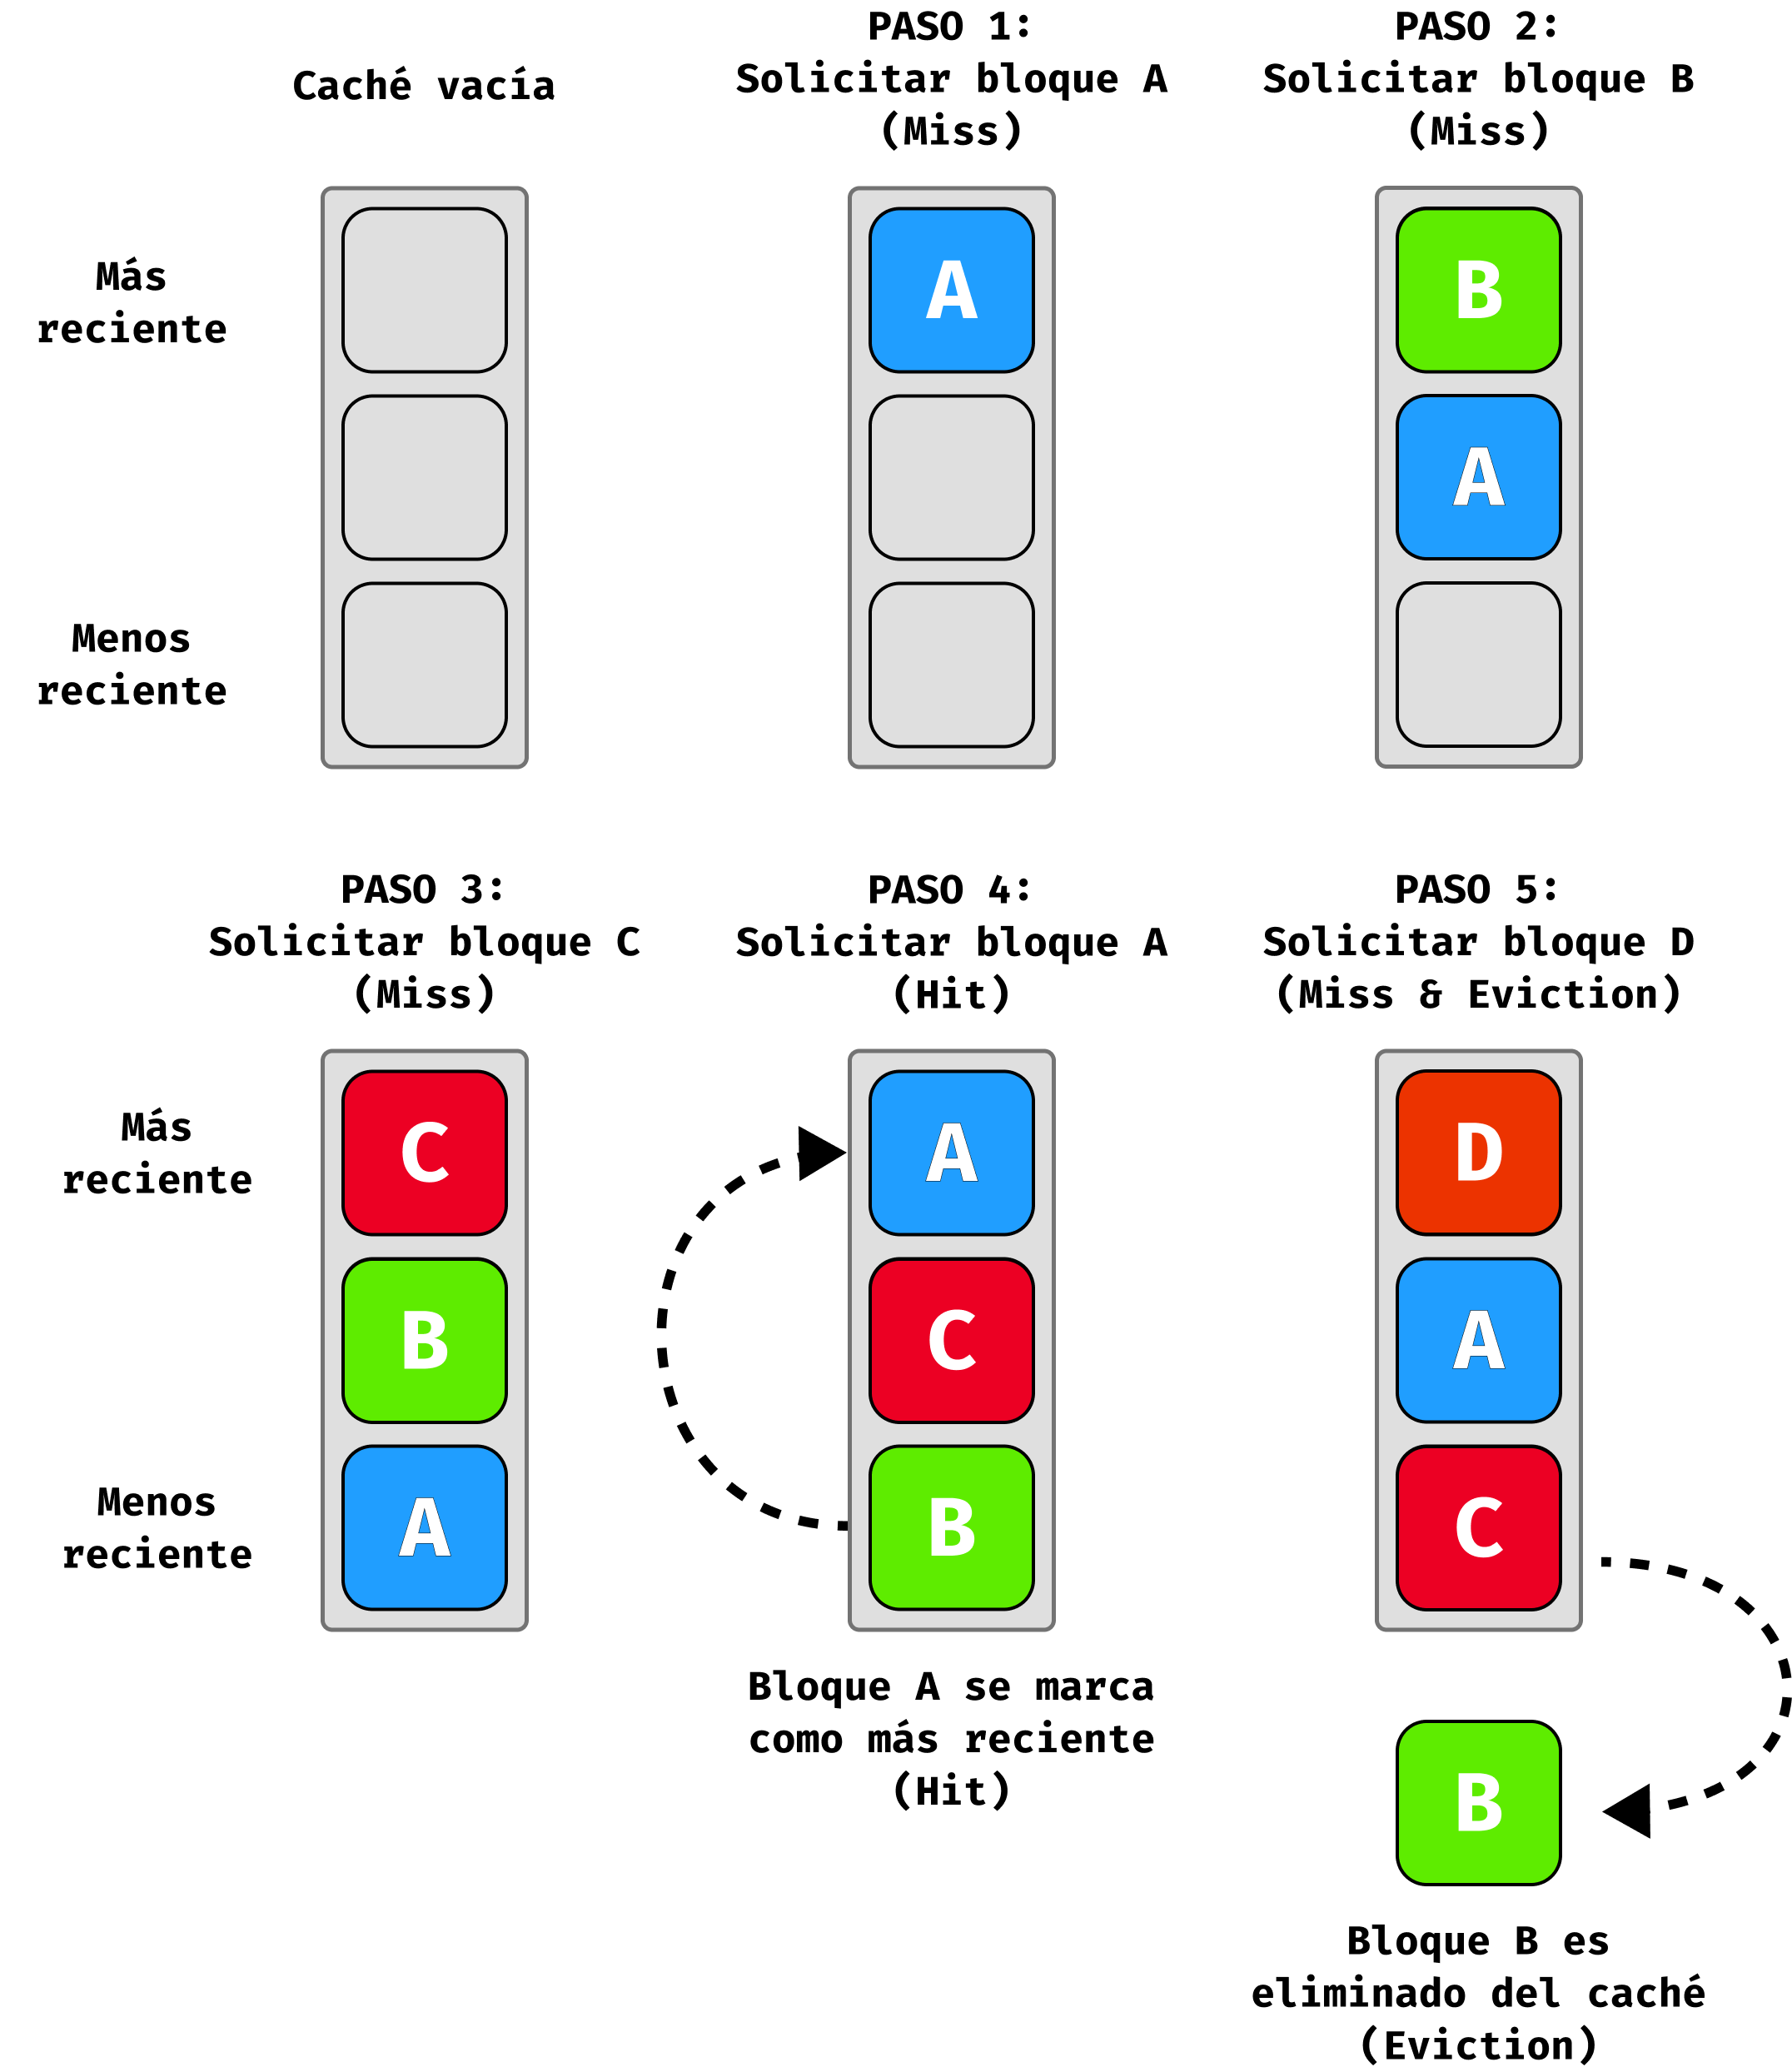
\includegraphics[width=.62\textwidth]{lru-cache.png}
  \caption{Bounded dense cache for materialized blocks. Reuse is explicit; eviction is allowed only for clean blocks, while dirty blocks must be flushed before their slots can be reclaimed.}
  \label{fig:lru-cache}
\end{figure}

\subsection{States}

Each block descriptor occupies exactly one of three states.
\begin{itemize}[leftmargin=1.4em]
  \item \texttt{COMPRESSED}: no dense copy exists in cache; the payload stored in compressed form is current.
  \item \texttt{CACHED\_CLEAN}: a dense copy exists in cache and matches the compressed payload.
  \item \texttt{CACHED\_DIRTY}: a dense copy exists in cache and is newer than the compressed payload.
\end{itemize}

\subsection{Transitions}

The legal state transitions are fixed.
\begin{enumerate}[leftmargin=1.5em]
  \item \textbf{Load:} \texttt{COMPRESSED} $\rightarrow$ \texttt{CACHED\_CLEAN}. The backend allocates a cache slot and reconstructs the dense block from its compressed payload.
  \item \textbf{Mutate:} \texttt{CACHED\_CLEAN} $\rightarrow$ \texttt{CACHED\_DIRTY}. A gate kernel modifies at least one amplitude in the materialized block.
  \item \textbf{Flush:} \texttt{CACHED\_DIRTY} $\rightarrow$ \texttt{CACHED\_CLEAN}. The backend recompresses the dense block and overwrites the corresponding compressed payload.
  \item \textbf{Evict:} \texttt{CACHED\_CLEAN} $\rightarrow$ \texttt{COMPRESSED}. The dense slot is released while the payload remains current in compressed storage.
\end{enumerate}

No direct transition from \texttt{CACHED\_DIRTY} to \texttt{COMPRESSED} is legal. A dirty block must be flushed before its slot can be reused.

\subsection{Backend Invariants}

The implementation should enforce four invariants continuously.
\begin{description}[leftmargin=1.4em,style=nextline]
  \item[Index invariant.] Every logical amplitude index maps to exactly one block identifier and one local offset.
  \item[Authority invariant.] Each block has exactly one authoritative representation, determined by its state.
  \item[Cache-slot invariant.] A cache slot contains at most one block, and a materialized block occupies exactly one cache slot.
  \item[Flush invariant.] After a global flush, every block is either \texttt{COMPRESSED} or \texttt{CACHED\_CLEAN}, and compressed storage matches the full logical state.
\end{description}

These invariants are sufficient to preserve logical correctness throughout decompression, mutation, writeback, and eviction.

\section{Block Acquisition, Eviction, and Writeback}

A compressed backend is implementable only if block acquisition is deterministic. The procedure below is the core of the design.

\subsection{AcquireBlock$(j)$}

For a logical block identifier $j$, the backend executes the following steps.
\begin{enumerate}[leftmargin=1.5em]
  \item Read descriptor $D_j$.
  \item If $D_j.\mathrm{state}\in\{\texttt{CACHED\_CLEAN},\texttt{CACHED\_DIRTY}\}$, refresh replacement metadata and return the address of its dense cache slot.
  \item Otherwise select a free cache slot; if no free slot exists, select a victim according to the replacement policy.
  \item If the victim block is dirty, flush it: compress the dense slot, overwrite the victim payload in the backing store, and update the victim descriptor to \texttt{CACHED\_CLEAN}.
  \item Evict the clean victim by clearing its cache-slot mapping and changing its state to \texttt{COMPRESSED}.
  \item Decompress block $j$ into the selected slot, store the slot identifier in $D_j$, set $D_j.\mathrm{state}=\texttt{CACHED\_CLEAN}$, refresh replacement metadata, and return the slot.
\end{enumerate}

This procedure is the only legal way to obtain a dense view of a compressed block.

\subsection{Dirty Marking}

After a dense kernel writes to a block, the backend sets the corresponding descriptor to \texttt{CACHED\_DIRTY}. No recompression is forced immediately. Delayed writeback is essential because consecutive gates often reuse the same working set, and recompressing after every update would destroy locality.

\subsection{FlushDirty$(S)$}

Given a set of materialized dirty blocks $S$, the backend flushes each block using the same steps.
\begin{enumerate}[leftmargin=1.5em]
  \item Read the dense data from its cache slot.
  \item Apply any reversible preprocessing required by the selected codec.
  \item Compress the block.
  \item Write the payload to the backing store and update offset and payload length metadata if needed.
  \item Change the descriptor state from \texttt{CACHED\_DIRTY} to \texttt{CACHED\_CLEAN}.
\end{enumerate}

A full synchronization flush simply applies \texttt{FlushDirty} to all dirty blocks currently resident in cache.

\section{Gate Planning Over the Block Layout}

The simulator still emits logical gates, but the backend must convert each gate invocation into a block-access plan before the dense kernel runs.

\subsection{Single-Qubit Pair Structure}

A single-qubit gate acting on target qubit $q$ updates amplitude pairs $(i, i \oplus 2^q)$ for all indices $i$ whose $q$-th bit is zero~\cite{Nielsen2010}. The stride of the pair relation is therefore
\begin{equation}
  s(q)=2^q.
\end{equation}
For a block size $B=2^b$, the target qubit immediately determines whether pair partners remain inside one block.

\textbf{Proposition 1.} If $q<b$, every pair $(i,i\oplus 2^q)$ remains within a single block. If $q\geq b$, cross-block pairs occur.

\textit{Reason.} A block boundary appears every $2^b$ consecutive logical indices. Flipping bit $q<b$ changes only lower-order bits inside the boundary interval, while flipping bit $q\geq b$ changes a bit that contributes to the block number.

This proposition is operational: it tells the backend whether one block view is enough or whether several blocks must be acquired together.

\subsection{Execution Plans}

The backend benefits from classifying gate invocations into execution plans.

\paragraph{Intra-block plan.}
Used when every touched pair lies inside one block. The backend iterates block by block:
\begin{enumerate}[leftmargin=1.5em]
  \item acquire one block,
  \item apply the dense kernel to the local offsets involved in that block,
  \item mark the block dirty,
  \item continue with the next logical block.
\end{enumerate}
This is the cheapest path because only one materialization is needed per active block.

\paragraph{Inter-block plan.}
Used when the pair relation spans two or more blocks in a regular pattern. The backend groups logical pair partners by block identifier, acquires the required block set, executes the dense kernel over those slot addresses, and marks each modified block dirty. A practical implementation should acquire the full group before kernel execution so that the dense kernel sees stable addresses for the whole update.

\paragraph{Generic multi-block plan.}
Used for broader access patterns such as arbitrary multi-qubit kernels. The backend builds the set of required logical blocks from the index map induced by the gate, acquires all of them, and dispatches a kernel that reads and writes through local offsets into the acquired block views. The same authority and dirty rules remain unchanged.

\subsection{Controlled Gates}

Controlled single-qubit gates keep the same target-driven pair relation as their uncontrolled counterpart and simply filter the active pair set using the control-mask condition. They therefore reuse the same planning logic: determine the partner stride from the target qubit, decide whether the access is intra-block or inter-block, acquire the required blocks, and apply the dense kernel only to logical pairs that satisfy the control predicate.

\subsection{Two-Qubit and Larger Kernels}

A two-qubit gate affects amplitude groups indexed by two target bits instead of one. The backend does not need a separate storage model for this case. It needs only two planning steps:
\begin{enumerate}[leftmargin=1.5em]
  \item enumerate the logical indices touched by one kernel application pattern;
  \item map those indices through $(j(i),o(i))$ to obtain the required block set and local offsets.
\end{enumerate}
If all mapped indices fall in one logical block, the operation becomes a local block kernel. Otherwise it becomes a multi-block kernel using the generic plan.

\section{Compression Pipeline and Backing Store}

The architecture is compatible with several block codecs, including floating-point compressors and reversible preprocessing schemes~\cite{burtscher2009fpc,lindstrom2006fpzip,masui2015bitshuffle}. The backend should treat the codec as a pluggable stage behind one fixed block contract.

\subsection{Per-Block Pipeline}

For each block, the physical write path is:
\begin{center}
  dense amplitudes $\rightarrow$ optional reversible transform $\rightarrow$ compression $\rightarrow$ payload write.
\end{center}
The read path is the inverse:
\begin{center}
  payload read $\rightarrow$ decompression $\rightarrow$ inverse transform $\rightarrow$ dense amplitudes.
\end{center}

The simulator never observes this pipeline. It requests block views; the backend decides how those views are reconstructed.

\subsection{Backing Store Layout}

An implementation can store compressed payloads in memory, on local disk, or in another backing medium. The architecture only requires that each block descriptor identifies where its current payload is stored and how long it is. Variable compressed sizes are expected, so the descriptor must support payload relocation after recompression. A practical storage manager can satisfy this requirement with either:
\begin{itemize}[leftmargin=1.4em]
  \item an append-only payload region plus updated offsets, or
  \item a reusable free-space map for overwritten payload regions.
\end{itemize}

The architectural requirement is simple: the descriptor for block $j$ must always point to the unique current payload of that block whenever the block is not dirty in cache.

\section{Synchronization and State Export}

At any point during execution, dirty cached blocks may contain newer data than compressed storage. The backend therefore needs explicit synchronization points where compressed storage is brought back into agreement with the logical state.

\subsection{Synchronization Events}

An implementation should synchronize at least on the following events.
\begin{itemize}[leftmargin=1.4em]
  \item Before exporting the full state vector.
  \item Before serializing the compressed state as a stable checkpoint.
  \item Before releasing backend resources at the end of simulation.
  \item Before any operation that requires the compressed store itself to be globally current.
\end{itemize}

\subsection{Correctness Statement}

\textbf{Proposition 2.} If the index invariant, authority invariant, cache-slot invariant, and flush invariant hold, then the compressed backend is logically equivalent to a dense state-vector backend.

\textit{Reason.} Every logical amplitude belongs to one unique block and local offset. Every kernel update is applied to the dense materialization of the unique block set that contains those logical amplitudes. After mutation, the updated dense copy is authoritative until writeback. A synchronization flush restores compressed storage to the same logical values. Therefore every logical read, gate result, and exported state matches the result of a dense implementation.

The proposition is enough for implementation: correctness depends on obeying the acquisition, dirty, flush, and eviction rules, not on any special property of the codec beyond exact block reconstruction.

\section{Implementation Guidance and Design Choices}

The architecture leaves room for engineering choices, but some choices are more important than others because they change runtime behavior directly.

\begin{table}
\centering
\small
\caption{Primary design parameters and their implementation effect.}
\label{tab:design-parameters}
\begin{tabular}{>{\raggedright\arraybackslash}p{.22\textwidth}
                >{\raggedright\arraybackslash}p{.28\textwidth}
                >{\raggedright\arraybackslash}p{.38\textwidth}}
\toprule
\textbf{Parameter} & \textbf{Implementation role} & \textbf{Practical effect} \\
\midrule
Block size $B$ & Defines partition granularity. & Larger blocks often compress better and favor local execution for more gates; smaller blocks reduce miss cost and metadata locality. \\
Cache capacity $C$ & Bounds dense residency. & Small caches increase decompression frequency; large caches approach dense storage behavior. \\
Replacement policy & Chooses the eviction victim. & LRU is simple and exploits temporal locality in repeated block use. \\
Codec choice & Defines block compression time and ratio. & Fast codecs reduce latency; stronger codecs may reduce the footprint further. \\
Writeback timing & Chooses when dirty blocks are recompressed. & Delayed writeback improves reuse; frequent flushes simplify memory turnover. \\
Backing-store manager & Tracks payload locations. & Needed because block payload sizes vary after recompression. \\
\bottomrule
\end{tabular}
\end{table}

Two implementation recommendations follow directly from the architecture.

First, cache and block metadata should be updated in one place only, ideally in the acquisition and flush routines. Centralizing those transitions keeps the authority rule simple and makes debugging feasible.

Second, gate planning should be separated from gate arithmetic. The planner computes the block set and local offsets; the dense kernel only consumes dense pointers and local index lists. This separation allows the simulator to reuse existing dense kernels while replacing only the storage and scheduling layer.

\section{Related Work}

Dense state-vector simulators remain the reference model for exact quantum circuit execution and expose the memory bottleneck that motivates the present design~\cite{Jones2019,Steiger2018,Haner2017,diaz2024software,diaz_mdpi_mmss}. Alternative representations such as tensor networks and decision diagrams reduce memory by changing the representation itself~\cite{Vidal2003,Markov2008,Vinkhuijzen2023}. The architecture developed here stays within the conventional state-vector model and instead reorganizes how that model is stored and recovered.

Compression-assisted simulation has already shown that amplitude data can sometimes be stored more compactly and that compression ratio depends strongly on the circuit family and on the numerical structure of the simulated state~\cite{wu2018amplitude,wu2019full,Zhang2025BMQSim}. The present work addresses a different layer of the problem: not whether compression can help, but how a simulator backend must be structured so that compressed storage can safely serve as the primary execution-time representation. The key architectural elements are contiguous block partitioning, a unique authority rule per block, bounded dense materialization, explicit dirty writeback, and gate planning over the induced block layout.

\section{Conclusion}

This paper presented a compressed-block backend architecture for full-state quantum circuit simulation at the level of direct implementation. The design keeps a logical dense state-vector interface for the simulator while storing the physical state as independent compressed blocks plus a bounded cache of dense materializations. Its core mechanisms are the logical-to-physical index map, the block descriptor, the three-state cache machine, the deterministic acquisition protocol, and the gate planner that converts logical gate semantics into block-local execution plans.

The value of the architecture is practical clarity. A developer implementing compressed execution for a Schr\"odinger-style simulator needs to decide how blocks are represented, when dense views are created, how stale compressed payloads are avoided, and how gate access traverses the block layout. Those decisions are made explicit here as backend rules and structures, so the compressed representation becomes a controllable execution substrate rather than an external storage add-on.

\begin{credits}
\subsubsection{\ackname}
This work is part of an undergraduate research project at Universidad Industrial de Santander on memory management for software quantum simulators.

\subsubsection{\discintname}
The authors have no competing interests to declare that are relevant to the content of this article.
\end{credits}

\bibliographystyle{splncs04}
\bibliography{references}

\end{document}
